%!TeX root = MOSFET_driver
\documentclass[main.tex]{subfiles}

\begin{document}
    \section{MOSFET driver}
    \justify
    While the availability of N-channel MOSFET drivers for both high-side and low-side is abundance, those for P-channel MOSFET are difficult to source. Thus, in this project, a driver circuit has to be designed and built. In this section, the followings are discussed:
    \begin{enumerate}
        \item MOSFET basic switching circuit
        \item Push-pull topology.
        \item Totem pole alternative topology.
    \end{enumerate}   

    \pagebreak
    \subsection{MOSFET basic switching circuit} 
    
    An example driver circuit for P-channel MOSFET is shown in Figure \ref{fig:ideal_gate_drive}. In this circuit, the gate is charged with an ideal power supply. The Zener diode $D1$ connected across the Source-Gate clamps the voltage at the diode zener breakdown voltage which is lower than the specified maximum $V_{gs\_max}$. In Figure \ref{fig:single_transistor_gate_drive}, a transistor is used to allows the small voltage control from device such as MCU, op-amp, etc.

    \begin{figure}[!h]
        \centerline{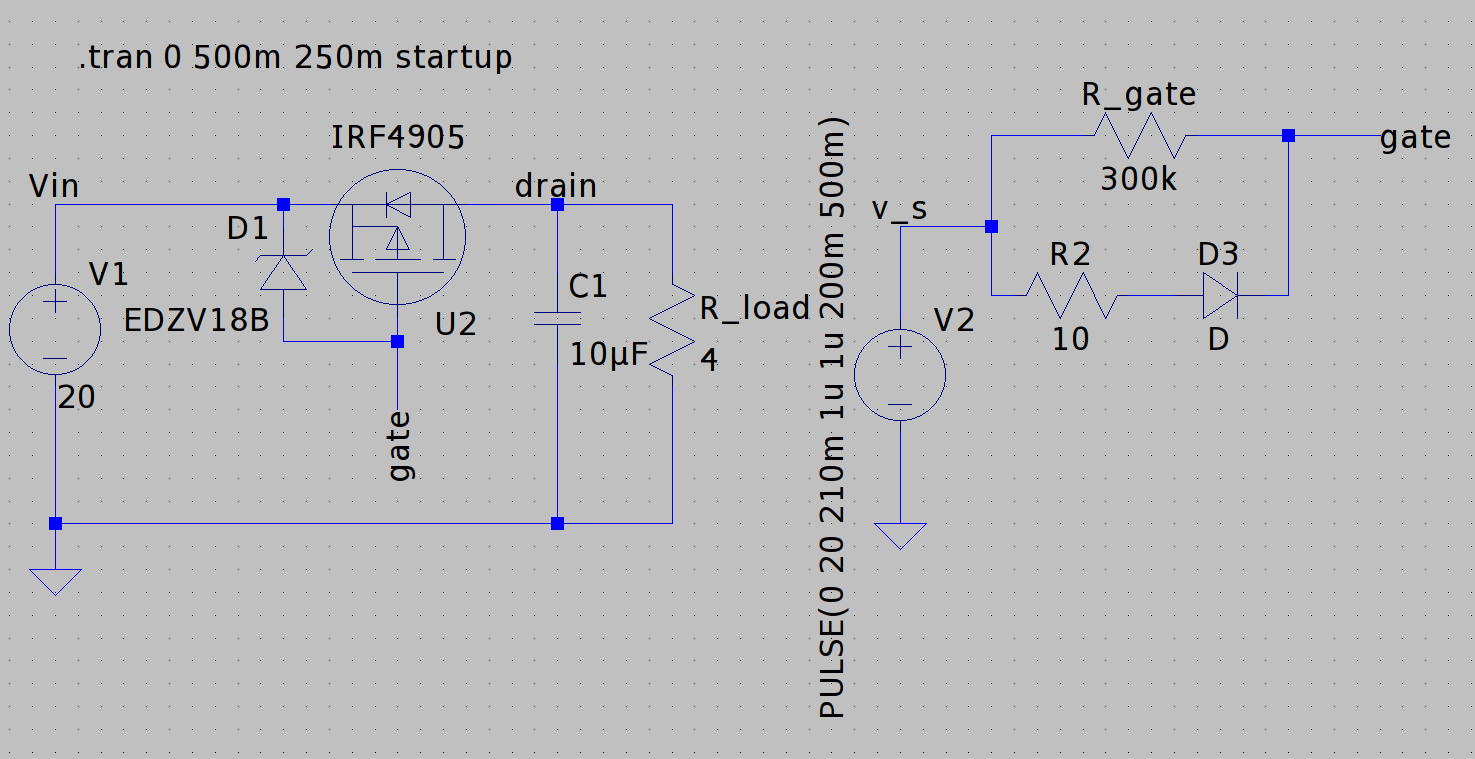
\includegraphics[width=\linewidth]{media/ideal_gate_drive.png}}
        \caption{Ideal gate driver circuit.}
        \label{fig:ideal_gate_drive}
    \end{figure}

    \begin{figure}[!h]
        \centerline{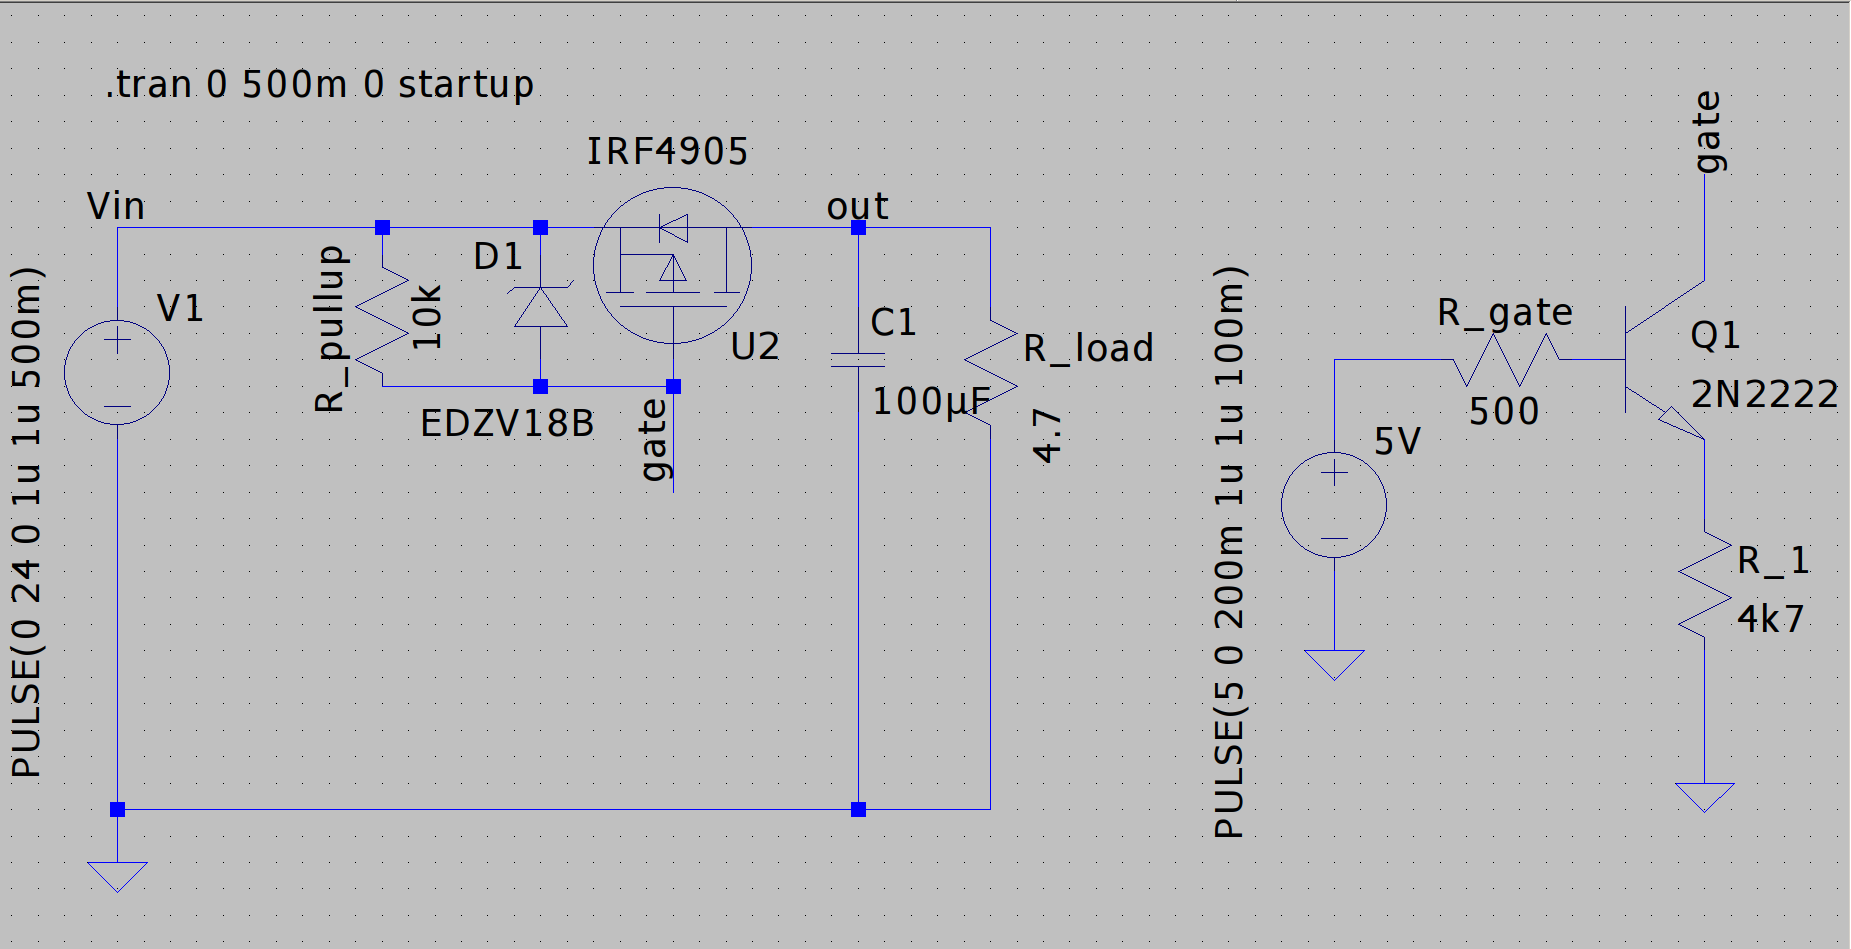
\includegraphics[width=\linewidth]{media/pmos_switch_npn.png}}
        \caption{Single-transistor gate driver circuit.} 
        \label{fig:single_transistor_gate_drive}
    \end{figure}

    \justify
    From the two example circuit, the following remarks can be made:
    \begin{enumerate}
        \item In the ideal example, the diode $D3$ allows for a larger current to be used for charging the gate which makes the turn-off event faster than turn-on (slow turn-on). This effect is desirable for application with capacitive load to reduce in-rush current.

        \item To replicate the slow turn-on effect in the single-transistor gate driver, the current through the $R_{pullup}$ while $Q_1$ is cut-off needs to be larger than that while $Q_1$ is in ohmic/saturation region, represented by equation \eqref{eq:slow_turn_on_condition}. This is generally plausible if the BJT is designed to be saturation region when turned on.
        
        \begin{equation} \label{eq:slow_turn_on_condition}
            I_{pullup}(\textbf{cut-off}) > I_{pullup}(\textbf{on})
        \end{equation}

        \item In MOSFET design, for a turn-on event, it is common to design to satisfy the following equation. It is so that the MOSFET is guaranteed to be in saturation region across the operating voltages.
        \begin{equation}
            V_{gs} \approx -V_{in}
        \end{equation}

        Which leads to the following equation:

        \begin{equation} \label{eq:deep_saturation_condition}
            R_{E1} << R_{pullup} \Longleftrightarrow I_{pullup}(\textbf{cut-off}) > I_{pullup}(\textbf{on})
        \end{equation}
        
    \end{enumerate}

    \justify
    Equation \eqref{eq:slow_turn_on_condition} and \eqref{eq:deep_saturation_condition} are conflicting and cannot be achieved in the single-transistor gate driver. Thus, a push-pull topology or similar derivative can be used.

    \pagebreak
    \subsection{Push-pull topology}

    \justify
    A push-pull topology uses a pair of transistors, one sinking current (pull-down), and the other sourcing current (pull-up).
    
    \pagebreak

    \section{Overvoltage/Undervoltage Protection}

    \subsection{Overvoltage protection}

    \justify
    Reference schematic:

    \begin{figure}[!h]
        \centerline{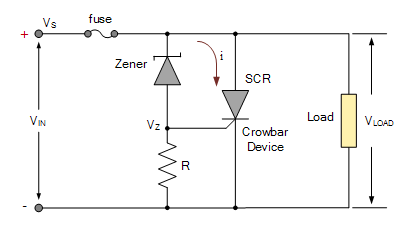
\includegraphics[scale=0.5]{media/Zener_Crowbar_OVP.png}}
        \caption{Electrical box arrangement overview.}
        \label{fig:enclosure_arrange}
    \end{figure}
    
\end{document}